\documentclass{article}
\usepackage{amsmath,tikz}

\begin{document}
\section{Gradient Descent}
\subsection{Finite difference}
using finite difference to get derivative of cost function
\begin{align}
  C'(w) = \lim_{\epsilon \to 0 }\frac{C(w+\epsilon)-C(w)}\epsilon
\end{align}

\subsection{Linear Model}
\begin{center}
	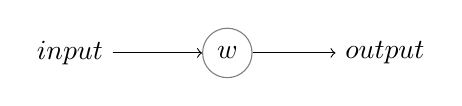
\begin{tikzpicture}
		\node (X) at (-2,0) {$input$};
		\node (F) [shape=circle,draw=gray] at (0,0) {$w$};
		\node (Y) at (2,0) {$output$};
		\path[->] (X) edge (F);
		\path[->] (F) edge (Y);
	\end{tikzpicture}
\end{center}
\begin{align}
	y = w * x
\end{align}

\subsubsection{Cost}
\begin{align}
	C(w) &= \frac{1}{n}\sum_{i=1}^{n}(x_iw -y_i)^2 	\\
	C'(w) &= \left(\frac{1}{n}\sum_{i=1}^{n}(x_iw -y_i)^2\right)' \\
	&=\frac{1}{n}\left(\sum_{i=1}^{n}(x_iw -y_i)^2\right)' \\
	&=\frac{1}{n}\left((x_1w-y_1)^2+\hdots+(x_nw-y_n)^2\right)' \\
	&=\frac{1}{n}\left((x_1w-y_1)+\hdots+(x_nw-y_n)\right)' \\
 &=  \frac{1}{n}\sum_{i=1}^{n}2x_i(x_iw -y_i)\\
	&=  \frac{2}{n}\sum_{i=1}^{n}x_i(x_iw -y_i)
\end{align}

\subsection{One Neuron Model with 2 inputs}
\begin{center}
	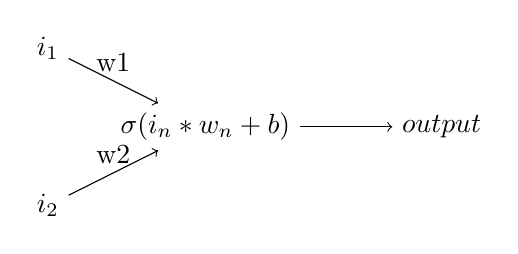
\begin{tikzpicture}
		\node (input1) at (-2,1) {$i_1$};
		\node (input2) at (-2,-1) {$i_2$};
		\node (F)  at (0,0) {$\sigma(i_n*w_n+b)$};
		\node (Y) at (3,0) {$output$};
		\path[->] (input1)  edge node[above] {w1} (F);
		\path[->] (input2)  edge node[above] {w2} (F);
		\path[->] (F) edge (Y);
	\end{tikzpicture}
	
\end{center}
\begin{align}
	output &=  y = \sigma(i_1*w1+i_2*w2 +b)  \\
	\sigma(x) &= \frac{1}{1+e^{-x}} \\
	\sigma'(x) &= \sigma(x)(1 -\sigma(x))
\end{align}

\subsubsection{Cost}

\def\pd[#1]{\partial_{#1}}
\def\avgsum[#1,#2]{\frac{1}{#2}\sum_{#1=1}^{#2}}

\begin{align}
	a_i &= \sigma(i_1*w1+i_2*w2 +b) \\
	\partial_{w_1} a_i  &= \partial_{w_1}( \sigma(i_1*w1+i_2*w2 +b) ) \\
	&= a_i(1-a_i)\partial_{w_1}(i_1w_1+i_2w_2 + b) \\
	&=a_i(1-a_i)i_1 \\
\partial_{w_2} a_i  &= \partial_{w_2}( \sigma(i_1*w1+i_2*w2 +b) ) \\
&= a_i(1-a_i)\partial_{w_2}(i_1w_1+i_2w_2 + b) \\
&=a_i(1-a_i)i_2 \\
\partial_{b} a_i  &= \partial_{b}(\sigma(i_1w_1+i_2w_2 + b)) \\
&=a_i(1-a_i) \\
(z_i :  \text{expected output}) \\
  C &= \avgsum[i, n](a_i - z_i)^2 \\
\pd[w_1] C
&= \avgsum[i, n]\pd[w_1]\left((a_i - z_i)^2\right) = \\
&= \avgsum[i, n]2(a_i - z_i)\pd[w_1]a_i = \\
&= \avgsum[i, n]2(a_i - z_i)a_i(1 - a_i)i_1 \\
\pd[w_2] C &= \avgsum[i, n]2(a_i - z_i)a_i(1 - a_i)i_2 \\
\pd[b] C &= \avgsum[i, n]2(a_i - z_i)a_i(1 - a_i)
\end{align}

\subsection{Two Neurons Model with 1 input}

\def\d{2.0}

\begin{center}
	\begin{tikzpicture}
		\node (X) at (-\d, 0) {$x$};
		\node[shape=circle,draw=black] (N1) at (0, 0) {$\sigma, b^{(1)}$};
		\node[shape=circle,draw=black] (N2) at (\d, 0) {$\sigma, b^{(2)}$};
		\node (Y) at ({2*\d}, 0) {$y$};
		\path[->] (X) edge node[above] {$w^{(1)}$} (N1);
		\path[->] (N1) edge node[above] {$w^{(2)}$} (N2);
		\path[->] (N2) edge (Y);
	\end{tikzpicture}
\end{center}

\begin{align}
	a^{(1)} &= \sigma(xw^{(1)} + b^{(1)}) \\
	y &= \sigma(a^{(1)}w^{(2)} + b^{(2)})
\end{align}

The superscript in parenthesis denotes the current layer. For example $a_i^{(l)}$ denotes the activation from the $l$-th layer on $i$-th sample.

\subsubsection{Feed-Forward}

\begin{align}
	a_i^{(1)} &= \sigma(x_iw^{(1)} + b^{(1)}) \\
	\pd[w^{(1)}]a_i^{(1)} &= a_i^{(1)}(1 - a_i^{(1)})x_i \\
	\pd[b^{1}]a_i^{(1)} &= a_i^{(1)}(1 - a_i^{(1)}) \\
	a_i^{(2)} &= \sigma(a_i^{(1)}w^{(2)} + b^{(2)}) \\
	\pd[w^{(2)}]a_i^{(2)} &= a_i^{(2)}(1 - a_i^{(2)})a_i^{(1)} \\
	\pd[b^{(2)}]a_i^{(2)} &= a_i^{(2)}(1 - a_i^{(2)}) \\
	\pd[a_i^{(1)}]a_i^{(2)} &= a_i^{(2)}(1 - a_i^{(2)})w^{(2)}
\end{align}

\subsubsection{Back-Propagation}

\begin{align}
	C^{(2)} &= \avgsum[i, n] (a_i^{(2)} - y_i)^2 \\
	\pd[w^{(2)}] C^{(2)}
	&= \avgsum[i, n] \pd[w^{(2)}]((a_i^{(2)} - y_i)^2)  \\
	&= \avgsum[i, n] 2(a_i^{(2)} - y_i)\pd[w^{(2)}]a_i^{(2)}  \\
	&= \avgsum[i, n] 2(a_i^{(2)} - y_i)a_i^{(2)}(1 - a_i^{(2)})a_i^{(1)} \\
	\pd[b^{(2)}] C^{(2)} &= \avgsum[i, n] 2(a_i^{(2)} - y_i)a_i^{(2)}(1 - a_i^{(2)}) \\
	\pd[a_i^{(1)}]C^{(2)} &= \avgsum[i, n] 2(a_i^{(2)} - y_i)a_i^{(2)}(1 - a_i^{(2)})w^{(2)} \\
	e_i &= a_i^{(1)} - \pd[a_i^{(1)}]C^{(2)} \\
	C^{(1)} &= \avgsum[i, n] (a_i^{(1)} - e_i)^2 \\
	\pd[w^{(1)}]C^{(1)}
	&= \pd[w^{(1)}]\left(\avgsum[i, n] (a_i^{(1)} - e_i)^2\right) \\
	&= \avgsum[i, n] \pd[w^{(1)}]\left((a_i^{(1)} - e_i)^2\right) \\
	&= \avgsum[i, n] 2(a_i^{(1)} - e_i)\pd[w^{(1)}]a_i^{(1)} \\
	&= \avgsum[i, n] 2(\pd[a_i^{(1)}]C^{(2)})a_i^{(1)}(1 - a_i^{(1)})x_i \\
	\pd[b^{1}]C^{(1)} &= \avgsum[i, n] 2(\pd[a_i^{(1)}]C^{(2)})a_i^{(1)}(1 - a_i^{(1)})
\end{align}

\subsection{Arbitrary Neurons Model with 1 input}

Let's assume that we have $m$ layers.

\subsubsection{Feed-Forward}

Let's assume that $a_i^{(0)}$ is $x_i$.

\begin{align}
	a_i^{(l)} &= \sigma(a_i^{(l-1)}w^{(l)} + b^{(l)}) \\
	\pd[w^{(l)}]a_i^{(l)} &= a_i^{(l)}(1 - a_i^{(l)})a_i^{(l-1)} \\
	\pd[b^{(l)}]a_i^{(l)} &= a_i^{(l)}(1 - a_i^{(l)}) \\
	\pd[a_i^{(l-1)}]a_i^{(l)} &= a_i^{(l)}(1 - a_i^{(l)})w^{(l)}
\end{align}

\subsubsection{Back-Propagation}

Let's denote $a_i^{(m)} - y_i$ as $\pd[a_i^{(m)}]C^{(m+1)}$.

\begin{align}
	C^{(l)} &= \avgsum[i, n] (\pd[a_i^{(l)}]C^{(l+1)})^2 \\
	\pd[w^{(l)}]C^{(l)} &= \avgsum[i, n] 2(\pd[a_i^{(l)}]C^{(l+1)})a_i^{(l)}(1 - a_i^{(l)})a_i^{(l-1)} \\
	\pd[b^{(l)}]C^{(l)} &= \avgsum[i, n] 2(\pd[a_i^{(l)}]C^{(l+1)})a_i^{(l)}(1 - a_i^{(l)}) \\
	\pd[a_i^{(l-1)}]C^{(l)} &= \avgsum[i, n] 2(\pd[a_i^{(l)}]C^{(l+1)})a_i^{(l)}(1 - a_i^{(l)})w^{(l)}
\end{align}


\end{document}